\newpage
\section{37. 解数独}
\label{leetcode:37}

\subsection{题目}

编写一个程序,通过已填充的空格来解决数独问题。

一个数独的解法需遵循如下规则:

\begin{enumerate}
  \item 数字 1-9 在每一行只能出现一次。
  \item 数字 1-9 在每一列只能出现一次。
  \item 数字 1-9 在每一个以粗实线分隔的 3x3 宫内只能出现一次。
\end{enumerate}

空白格用 \verb|'.'| 表示。

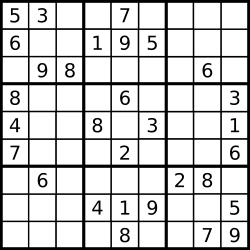
\includegraphics[width=60mm,height=60mm]{images/leetcode/37_sudo.png}

一个数独。

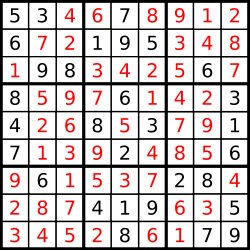
\includegraphics[width=60mm,height=60mm]{images/leetcode/37_sudo_solution.png}

答案被标成红色。

\textbf{Note}:

\begin{itemize}
  \item 给定的数独序列只包含数字 1-9 和字符 \verb|'.'| 。
  \item 你可以假设给定的数独只有唯一解。
  \item 给定数独永远是 9x9 形式的。
\end{itemize}

\subsection{参考题解}

\subsubsection{Python}

\begin{verbatim}
class Solution:
  def solveSudoku(self, board: List[List[str]]) -> None:
    """
    Do not return anything, modify board in-place instead.
    """
    self.board = board
    self.rows = len(board)
    self.cols = len(board[0])
    self.solve()

  def solve(self):
    for row in range(self.rows):
      for col in range(self.cols):
        if self.board[row][col] != ".":
          continue
        for num in ["1","2","3","4","5","6","7","8","9"]:
          if self.isValid(row, col, num):
            self.board[row][col] = num
            if self.solve():
              return True
            self.board[row][col] = "."
        return False
    return True

  def isValid(self, row, col, c):
    for i in range(9):
      if self.board[i][col] == c:
        return False
      if self.board[row][i] == c:
        return False
      if self.board[row // 3 * 3 + i // 3][col // 3 * 3 + i % 3] == c:
        return False
    return True
\end{verbatim}
